%!TEX root = tcc_proposta.tex

%----------------------------------------------------------------------------------
% Exemplo do uso da classe tcc.cls. Veja o arquivo .cls
% para mais detalhes e instruções.
%----------------------------------------------------------------------------------

% PARA PREENCHIMENTO DO REVISOR:
% CHECKLIST
% [ ] Introduction: check the introduction 
    % [ ] Avoid jargon: Do you avoid jargon that is only explain in the rest of the text?
    % [ ] Clarity: Can anyone from computer science read the introduction and understand what's the objective?
    % [ ] Does it clearly describe the problem?
    % [ ] Does the introduction clearly state the contributions?

\chapter{Introdução}\label{chap1:intro}
	Nos últimos anos, avanços significativos em robótica e em inteligência artificial contribuíram para que pesquisas no desenvolvimento de veículos de superfície aquática não tripulados (do inglês \textit{"Unmanned Surface Vehicle"} - USV) ganhassem atenção~\cite{Huang2020Ship}. Um USV é definido por atuar de forma autônoma através de um sistema embarcado ou controlado remotamente~\cite{Song2018Two-level}. Conduzidas por frentes militares, científicas e privadas, pesquisas no desenvolvimento de USVs têm o intuito de auxiliar em atividades como monitoramento, comércio, exploração e pesquisas~\cite{Jurak2020COLREGS}. Caso realizadas por um USV, as atividades citadas poderiam possuir uma maior duração e potencialmente maior acurácia, além de permitir redução do custo de manutenção~\cite{Liu2016Unmanned}. Porém, aspirar essa série de atividades para um USV fará com que sua atuação ocorra em cenários compartilhados com outras embarcações~\cite{Kuwata2014Safe}.

    Sob responsabilidade da Organização Internacional da Marinha (do inglês \textit{"International Marine Organization"} - IMO), as regulamentações de prevenção de colisões no mar (do inglês \textit{"COLlision REGulations at Sea"} - COLREGS) definem como as embarcações devem agir em situações de colisão~\cite{Jurak2020COLREGS}. Visto que investigações apontam que acidentes marítimos acontecem principalmente pela violação das COLREGS~\cite{Song2018Two-level}, é importante considerar a sua implementação no desenvolvimento de USVs. Dada a frequência de colisões e a gravidade das consequências, acidentes entre embarcações são uma preocupação latente~\cite{Huang2019Generalized}. Por conta disso, evasão de colisão é um dos aspectos fundamentais no desenvolvimento de USV~\cite{Jurak2020COLREGS}. 

    Apesar da necessidade de considerar COLREGS no desenvolvimento de USVs, elas foram pensadas para serem compreendidas por humanos, que podem condicionar a sua aplicação à cada caso~\cite{Kuwata2014Safe}. Na Figura~\ref{fig:Kuwata2014_colregsInterpretation}, conforme apresentada por Kuwata \etal~\cite{Kuwata2014Safe}, é possível observar uma situação onde há risco de colisão (Figura~\ref{fig:Kuwata2014_colregApplicable}) e, portanto, deve-se aplicar as COLREGS. Uma situação semelhante porém sem risco de colisão é apresentada na Figura~\ref{fig:Kuwata2014_colregNA}, onde as COLREGS não são aplicáveis pois, dado a velocidade das embarcações, não há risco de colisão. Para identificar situações em que as COLREGS devem, ou não, ser aplicadas é preciso identificar que há um risco de colisão. Para isso, se utiliza um Índice de Risco de Colisão (do inglês \textit{"Collision Risk Index"} - CRI)~\cite{Huang2019Generalized}. Esse índice pode ser obtido através do método Ponto de Maior Aproximação (do inglês \textit{"Closest Point of Approach"} - CPA), que utiliza indicadores, como "tempo para o ponto de maior proximidade" (do inglês \textit{"Time to Closest Point of Approach"} - TCPA) e "distância no ponto de maior proximidade" (do inglês \textit{"Distance to Closest Point of Approach"} - DCPA), para determinar se um determinado encontro apresenta risco de colisão ou não~\cite{Huang2020Ship}. 
    
    Este trabalho apresenta o desenvolvimento do CPA em um sistema base para USV desenvolvido por Jurak~\cite{Jurak2020COLREGS}. O presente documento está estruturado da seguinte forma: no Capítulo~\ref{chap2:fund_teo} apresentamos a metodologia, os conceitos e as técnicas utilizadas neste trabalho; no Capítulo~\ref{chap3:framework_desenvolvimento} introduzimos as ferramentas utilizadas no desenvolvimento deste trabalho, bem como uma descrição do sistema base desenvolvido por Jurak~\cite{Jurak2020COLREGS}; 
    no Capítulo~\ref{chap4:desenvolvimento} apresentamos o desenvolvimento; no Capítulo~\ref{chap5:resultados} apresentamos as análises dos resultados obtidos nos testes realizados, bem como uma comparação com os resultados do sistema base; no Capítulo~\ref{chap6:conclusao} discutimos os resultados obtidos e dissertamos a respeito dos trabalhos futuros.
    
    \begin{figure}
		\centering
        \begin{subfigure}{0.4\textwidth}
            \centering
            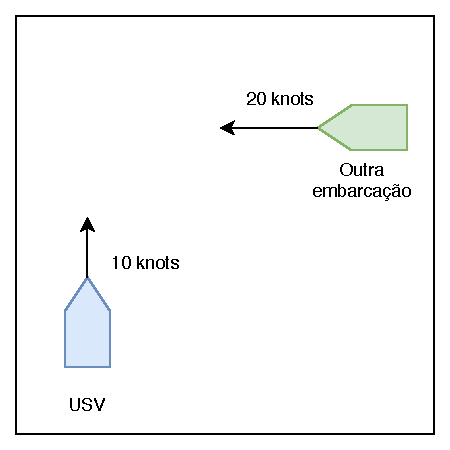
\includegraphics[width=\textwidth]{fig/chap1/kuwata_image_collision.pdf}
            \caption{}
            \label{fig:Kuwata2014_colregApplicable}
        \end{subfigure}
        \begin{subfigure}{0.4\textwidth}
            \centering
            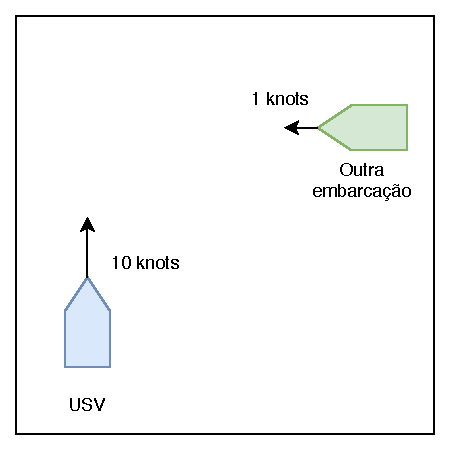
\includegraphics[width=\textwidth]{fig/chap1/kuwata_image_safe.pdf}
            \caption{}
            \label{fig:Kuwata2014_colregNA}
        \end{subfigure}
    
    \caption{Mesmo encontro para diferentes velocidades da embarcação que se aproxima. Na Figura~(a) a COLREGS é aplicável e o USV deve desviar da embarcação que se aproxima, enquanto que na Figura (b) a COLREGS não é aplicável e o USV pode seguir sua rota sem alteração.}
    \label{fig:Kuwata2014_colregsInterpretation}
    \end{figure}